\documentclass[twoside]{book}

% Packages required by doxygen
\usepackage{fixltx2e}
\usepackage{calc}
\usepackage{doxygen}
\usepackage[export]{adjustbox} % also loads graphicx
\usepackage{graphicx}
\usepackage[utf8]{inputenc}
\usepackage{makeidx}
\usepackage{multicol}
\usepackage{multirow}
\PassOptionsToPackage{warn}{textcomp}
\usepackage{textcomp}
\usepackage[nointegrals]{wasysym}
\usepackage[table]{xcolor}

% Font selection
\usepackage[T1]{fontenc}
\usepackage[scaled=.90]{helvet}
\usepackage{courier}
\usepackage{amssymb}
\usepackage{sectsty}
\renewcommand{\familydefault}{\sfdefault}
\allsectionsfont{%
  \fontseries{bc}\selectfont%
  \color{darkgray}%
}
\renewcommand{\DoxyLabelFont}{%
  \fontseries{bc}\selectfont%
  \color{darkgray}%
}
\newcommand{\+}{\discretionary{\mbox{\scriptsize$\hookleftarrow$}}{}{}}

% Page & text layout
\usepackage{geometry}
\geometry{%
  a4paper,%
  top=2.5cm,%
  bottom=2.5cm,%
  left=2.5cm,%
  right=2.5cm%
}
\tolerance=750
\hfuzz=15pt
\hbadness=750
\setlength{\emergencystretch}{15pt}
\setlength{\parindent}{0cm}
\setlength{\parskip}{3ex plus 2ex minus 2ex}
\makeatletter
\renewcommand{\paragraph}{%
  \@startsection{paragraph}{4}{0ex}{-1.0ex}{1.0ex}{%
    \normalfont\normalsize\bfseries\SS@parafont%
  }%
}
\renewcommand{\subparagraph}{%
  \@startsection{subparagraph}{5}{0ex}{-1.0ex}{1.0ex}{%
    \normalfont\normalsize\bfseries\SS@subparafont%
  }%
}
\makeatother

% Headers & footers
\usepackage{fancyhdr}
\pagestyle{fancyplain}
\fancyhead[LE]{\fancyplain{}{\bfseries\thepage}}
\fancyhead[CE]{\fancyplain{}{}}
\fancyhead[RE]{\fancyplain{}{\bfseries\leftmark}}
\fancyhead[LO]{\fancyplain{}{\bfseries\rightmark}}
\fancyhead[CO]{\fancyplain{}{}}
\fancyhead[RO]{\fancyplain{}{\bfseries\thepage}}
\fancyfoot[LE]{\fancyplain{}{}}
\fancyfoot[CE]{\fancyplain{}{}}
\fancyfoot[RE]{\fancyplain{}{\bfseries\scriptsize Generated by Doxygen }}
\fancyfoot[LO]{\fancyplain{}{\bfseries\scriptsize Generated by Doxygen }}
\fancyfoot[CO]{\fancyplain{}{}}
\fancyfoot[RO]{\fancyplain{}{}}
\renewcommand{\footrulewidth}{0.4pt}
\renewcommand{\chaptermark}[1]{%
  \markboth{#1}{}%
}
\renewcommand{\sectionmark}[1]{%
  \markright{\thesection\ #1}%
}

% Indices & bibliography
\usepackage{natbib}
\usepackage[titles]{tocloft}
\setcounter{tocdepth}{3}
\setcounter{secnumdepth}{5}
\makeindex

% Hyperlinks (required, but should be loaded last)
\usepackage{ifpdf}
\ifpdf
  \usepackage[pdftex,pagebackref=true]{hyperref}
\else
  \usepackage[ps2pdf,pagebackref=true]{hyperref}
\fi
\hypersetup{%
  colorlinks=true,%
  linkcolor=blue,%
  citecolor=blue,%
  unicode%
}

% Custom commands
\newcommand{\clearemptydoublepage}{%
  \newpage{\pagestyle{empty}\cleardoublepage}%
}

\usepackage{caption}
\captionsetup{labelsep=space,justification=centering,font={bf},singlelinecheck=off,skip=4pt,position=top}

%===== C O N T E N T S =====

\begin{document}

% Titlepage & ToC
\hypersetup{pageanchor=false,
             bookmarksnumbered=true,
             pdfencoding=unicode
            }
\pagenumbering{alph}
\begin{titlepage}
\vspace*{7cm}
\begin{center}%
{\Large Group 7\+: Human Obstacle Detector }\\
\vspace*{1cm}
{\large Generated by Doxygen 1.8.13}\\
\end{center}
\end{titlepage}
\clearemptydoublepage
\pagenumbering{roman}
\tableofcontents
\clearemptydoublepage
\pagenumbering{arabic}
\hypersetup{pageanchor=true}

%--- Begin generated contents ---
\chapter{Class Index}
\section{Class List}
Here are the classes, structs, unions and interfaces with brief descriptions\+:\begin{DoxyCompactList}
\item\contentsline{section}{\hyperlink{classData}{Data} \\*\hyperlink{classData}{Data} class includes methods to get the input data and a method to put bounging boxes around the detected humans }{\pageref{classData}}{}
\item\contentsline{section}{\hyperlink{classDetect}{Detect} \\*\hyperlink{classDetect}{Detect} class uses a pre-\/trained S\+VM model from open\+CV to detect humans in the input frames and return bounding box co-\/ordinates }{\pageref{classDetect}}{}
\item\contentsline{section}{\hyperlink{classDistance}{Distance} \\*\hyperlink{classDistance}{Distance} class to provide the pixel to SI units conversion as well as the Transformation between Camera frame and Robot frame }{\pageref{classDistance}}{}
\end{DoxyCompactList}

\chapter{File Index}
\section{File List}
Here is a list of all documented files with brief descriptions\+:\begin{DoxyCompactList}
\item\contentsline{section}{app/\hyperlink{Data_8cpp}{Data.\+cpp} \\*\hyperlink{classData}{Data} Class Definition }{\pageref{Data_8cpp}}{}
\item\contentsline{section}{app/\hyperlink{Detect_8cpp}{Detect.\+cpp} \\*\hyperlink{classDetect}{Detect} Class Definition }{\pageref{Detect_8cpp}}{}
\item\contentsline{section}{app/\hyperlink{Distance_8cpp}{Distance.\+cpp} \\*\hyperlink{classDistance}{Distance} Class Definition }{\pageref{Distance_8cpp}}{}
\item\contentsline{section}{include/\hyperlink{Data_8hpp}{Data.\+hpp} \\*\hyperlink{classData}{Data} Class Declaration }{\pageref{Data_8hpp}}{}
\item\contentsline{section}{include/\hyperlink{Detect_8hpp}{Detect.\+hpp} \\*\hyperlink{classDetect}{Detect} Class Declaration }{\pageref{Detect_8hpp}}{}
\item\contentsline{section}{include/\hyperlink{Distance_8hpp}{Distance.\+hpp} \\*\hyperlink{classDistance}{Distance} Class Declaration }{\pageref{Distance_8hpp}}{}
\item\contentsline{section}{test/\hyperlink{DataTest_8cpp}{Data\+Test.\+cpp} \\*\hyperlink{classData}{Data} Class Tests }{\pageref{DataTest_8cpp}}{}
\item\contentsline{section}{test/\hyperlink{DetectTest_8cpp}{Detect\+Test.\+cpp} \\*\hyperlink{classDetect}{Detect} Class Tests }{\pageref{DetectTest_8cpp}}{}
\item\contentsline{section}{test/\hyperlink{DistanceTest_8cpp}{Distance\+Test.\+cpp} \\*\hyperlink{classDistance}{Distance} Class Tests }{\pageref{DistanceTest_8cpp}}{}
\end{DoxyCompactList}

\chapter{Class Documentation}
\hypertarget{classData}{}\section{Data Class Reference}
\label{classData}\index{Data@{Data}}


\hyperlink{classData}{Data} class includes methods to get the input data and a method to put bounging boxes around the detected humans.  




{\ttfamily \#include $<$Data.\+hpp$>$}



Collaboration diagram for Data\+:
\nopagebreak
\begin{figure}[H]
\begin{center}
\leavevmode
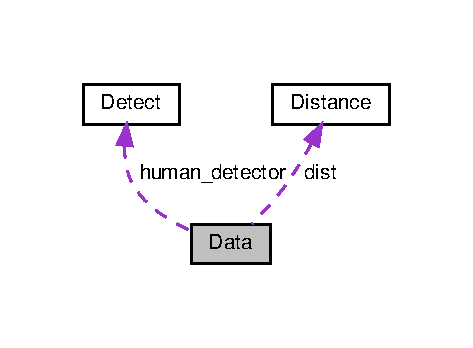
\includegraphics[width=227pt]{classData__coll__graph}
\end{center}
\end{figure}
\subsection*{Public Member Functions}
\begin{DoxyCompactItemize}
\item 
\mbox{\Hypertarget{classData_af11f741cb7f587e2e495452a8905a22a}\label{classData_af11f741cb7f587e2e495452a8905a22a}} 
\hyperlink{classData_af11f741cb7f587e2e495452a8905a22a}{Data} ()
\begin{DoxyCompactList}\small\item\em Construct a new \hyperlink{classData}{Data}\+:\+: \hyperlink{classData}{Data} object. \end{DoxyCompactList}\item 
int \hyperlink{classData_a511184f11597e720b0bf96b9b4f89a0b}{get\+Camera} (int mode)
\begin{DoxyCompactList}\small\item\em To take the camera frames as input. \end{DoxyCompactList}\item 
double \hyperlink{classData_a9875eec4b1ee3fc18512e5721513d34e}{load\+Video} (std\+::string file\+Path)
\begin{DoxyCompactList}\small\item\em To take frames from a video file as input frames. \end{DoxyCompactList}\item 
cv\+::\+Mat \hyperlink{classData_a8791dd62b1f57b4e4f2039e934ec7fdf}{pre\+Processing} (const cv\+::\+Mat \&frame)
\begin{DoxyCompactList}\small\item\em To resize and filter input images to operate on. \end{DoxyCompactList}\item 
cv\+::\+Mat \hyperlink{classData_ab0eefc277a688a36ec7bef63e8807bc2}{video\+Pre\+Processing} (const cv\+::\+Mat \&frame)
\begin{DoxyCompactList}\small\item\em To resize and filter input video frames to operate on. \end{DoxyCompactList}\item 
\mbox{\Hypertarget{classData_aab31956423290f0d62dcca47ab4d16dd}\label{classData_aab31956423290f0d62dcca47ab4d16dd}} 
\hyperlink{classData_aab31956423290f0d62dcca47ab4d16dd}{$\sim$\+Data} ()
\begin{DoxyCompactList}\small\item\em Destroy the \hyperlink{classData}{Data}\+:\+: \hyperlink{classData}{Data} object. \end{DoxyCompactList}\end{DoxyCompactItemize}
\subsection*{Public Attributes}
\begin{DoxyCompactItemize}
\item 
\mbox{\Hypertarget{classData_ae089cb20a02909129d8f055805d38f8e}\label{classData_ae089cb20a02909129d8f055805d38f8e}} 
\hyperlink{classDistance}{Distance} {\bfseries dist}
\item 
\mbox{\Hypertarget{classData_aa4b6fa81e2c1055e4a193bef4fd1b03c}\label{classData_aa4b6fa81e2c1055e4a193bef4fd1b03c}} 
\hyperlink{classDetect}{Detect} {\bfseries human\+\_\+detector}
\item 
\mbox{\Hypertarget{classData_aba335c8ce9ac25fe621238c4c5d9acdb}\label{classData_aba335c8ce9ac25fe621238c4c5d9acdb}} 
cv\+::\+Mat {\bfseries frame}
\end{DoxyCompactItemize}


\subsection{Detailed Description}
\hyperlink{classData}{Data} class includes methods to get the input data and a method to put bounging boxes around the detected humans. 

\subsection{Member Function Documentation}
\mbox{\Hypertarget{classData_a511184f11597e720b0bf96b9b4f89a0b}\label{classData_a511184f11597e720b0bf96b9b4f89a0b}} 
\index{Data@{Data}!get\+Camera@{get\+Camera}}
\index{get\+Camera@{get\+Camera}!Data@{Data}}
\subsubsection{\texorpdfstring{get\+Camera()}{getCamera()}}
{\footnotesize\ttfamily int Data\+::get\+Camera (\begin{DoxyParamCaption}\item[{int}]{mode }\end{DoxyParamCaption})}



To take the camera frames as input. 


\begin{DoxyParams}{Parameters}
{\em mode} & \+: Camera mode to view the camera or not \\
\hline
\end{DoxyParams}
\begin{DoxyReturn}{Returns}
int 
\end{DoxyReturn}
\mbox{\Hypertarget{classData_a9875eec4b1ee3fc18512e5721513d34e}\label{classData_a9875eec4b1ee3fc18512e5721513d34e}} 
\index{Data@{Data}!load\+Video@{load\+Video}}
\index{load\+Video@{load\+Video}!Data@{Data}}
\subsubsection{\texorpdfstring{load\+Video()}{loadVideo()}}
{\footnotesize\ttfamily double Data\+::load\+Video (\begin{DoxyParamCaption}\item[{std\+::string}]{file\+Path }\end{DoxyParamCaption})}



To take frames from a video file as input frames. 


\begin{DoxyParams}{Parameters}
{\em file\+Path} & Path to the video file \\
\hline
\end{DoxyParams}
\begin{DoxyReturn}{Returns}
double 
\end{DoxyReturn}
\mbox{\Hypertarget{classData_a8791dd62b1f57b4e4f2039e934ec7fdf}\label{classData_a8791dd62b1f57b4e4f2039e934ec7fdf}} 
\index{Data@{Data}!pre\+Processing@{pre\+Processing}}
\index{pre\+Processing@{pre\+Processing}!Data@{Data}}
\subsubsection{\texorpdfstring{pre\+Processing()}{preProcessing()}}
{\footnotesize\ttfamily cv\+::\+Mat Data\+::pre\+Processing (\begin{DoxyParamCaption}\item[{const cv\+::\+Mat \&}]{frame }\end{DoxyParamCaption})}



To resize and filter input images to operate on. 


\begin{DoxyParams}{Parameters}
{\em frame} & \+: Frame to be preprocessed \\
\hline
\end{DoxyParams}
\begin{DoxyReturn}{Returns}
cv\+::\+Mat 
\end{DoxyReturn}
\mbox{\Hypertarget{classData_ab0eefc277a688a36ec7bef63e8807bc2}\label{classData_ab0eefc277a688a36ec7bef63e8807bc2}} 
\index{Data@{Data}!video\+Pre\+Processing@{video\+Pre\+Processing}}
\index{video\+Pre\+Processing@{video\+Pre\+Processing}!Data@{Data}}
\subsubsection{\texorpdfstring{video\+Pre\+Processing()}{videoPreProcessing()}}
{\footnotesize\ttfamily cv\+::\+Mat Data\+::video\+Pre\+Processing (\begin{DoxyParamCaption}\item[{const cv\+::\+Mat \&}]{frame }\end{DoxyParamCaption})}



To resize and filter input video frames to operate on. 


\begin{DoxyParams}{Parameters}
{\em frame} & \+: Frame to be preprocessed \\
\hline
\end{DoxyParams}
\begin{DoxyReturn}{Returns}
cv\+::\+Mat 
\end{DoxyReturn}


The documentation for this class was generated from the following files\+:\begin{DoxyCompactItemize}
\item 
include/\hyperlink{Data_8hpp}{Data.\+hpp}\item 
app/\hyperlink{Data_8cpp}{Data.\+cpp}\end{DoxyCompactItemize}

\hypertarget{classDetect}{}\section{Detect Class Reference}
\label{classDetect}\index{Detect@{Detect}}


\hyperlink{classDetect}{Detect} class uses a pre-\/trained S\+VM model from open\+CV to detect humans in the input frames and return bounding box co-\/ordinates.  




{\ttfamily \#include $<$Detect.\+hpp$>$}

\subsection*{Public Member Functions}
\begin{DoxyCompactItemize}
\item 
\mbox{\Hypertarget{classDetect_afefa427dddf8e308f93fd49424cc3680}\label{classDetect_afefa427dddf8e308f93fd49424cc3680}} 
\hyperlink{classDetect_afefa427dddf8e308f93fd49424cc3680}{Detect} ()
\begin{DoxyCompactList}\small\item\em Construct a new \hyperlink{classDetect}{Detect}\+:\+: \hyperlink{classDetect}{Detect} object. \end{DoxyCompactList}\item 
std\+::vector$<$ double $>$ \hyperlink{classDetect_a7a27975d3aeb0ef43042106554fccb07}{detect\+Human} (cv\+::\+Mat \&input\+\_\+frame)
\begin{DoxyCompactList}\small\item\em Method to detect humans in input frames. \end{DoxyCompactList}\item 
std\+::vector$<$ double $>$ \hyperlink{classDetect_a67c037bd61725af5ec53beadcb4f58d0}{put\+Box} (cv\+::\+Mat \&input\+\_\+frame, std\+::vector$<$ double $>$ \&weights)
\begin{DoxyCompactList}\small\item\em Method to draw bouding boxes around detected humans. \end{DoxyCompactList}\item 
\mbox{\Hypertarget{classDetect_aa808b1146b9b8db316b25b02f0a6b5f3}\label{classDetect_aa808b1146b9b8db316b25b02f0a6b5f3}} 
\hyperlink{classDetect_aa808b1146b9b8db316b25b02f0a6b5f3}{$\sim$\+Detect} ()
\begin{DoxyCompactList}\small\item\em Destroy the \hyperlink{classDetect}{Detect}\+:\+: \hyperlink{classDetect}{Detect} object. \end{DoxyCompactList}\end{DoxyCompactItemize}
\subsection*{Public Attributes}
\begin{DoxyCompactItemize}
\item 
\mbox{\Hypertarget{classDetect_a26e995ab3b691ebf5f2ba2040aede421}\label{classDetect_a26e995ab3b691ebf5f2ba2040aede421}} 
std\+::vector$<$ cv\+::\+Rect $>$ {\bfseries box\+\_\+coordinates}
\item 
\mbox{\Hypertarget{classDetect_a7b4db15c556678a0f8e7ec1f925bd79d}\label{classDetect_a7b4db15c556678a0f8e7ec1f925bd79d}} 
cv\+::\+H\+O\+G\+Descriptor {\bfseries H\+OG}
\end{DoxyCompactItemize}


\subsection{Detailed Description}
\hyperlink{classDetect}{Detect} class uses a pre-\/trained S\+VM model from open\+CV to detect humans in the input frames and return bounding box co-\/ordinates. 

\subsection{Member Function Documentation}
\mbox{\Hypertarget{classDetect_a7a27975d3aeb0ef43042106554fccb07}\label{classDetect_a7a27975d3aeb0ef43042106554fccb07}} 
\index{Detect@{Detect}!detect\+Human@{detect\+Human}}
\index{detect\+Human@{detect\+Human}!Detect@{Detect}}
\subsubsection{\texorpdfstring{detect\+Human()}{detectHuman()}}
{\footnotesize\ttfamily std\+::vector$<$ double $>$ Detect\+::detect\+Human (\begin{DoxyParamCaption}\item[{cv\+::\+Mat \&}]{input\+\_\+frame }\end{DoxyParamCaption})}



Method to detect humans in input frames. 


\begin{DoxyParams}{Parameters}
{\em input\+\_\+frame} & \+:Frame to detect humans \\
\hline
\end{DoxyParams}
\begin{DoxyReturn}{Returns}
std\+::vector$<$double$>$ 
\end{DoxyReturn}
\mbox{\Hypertarget{classDetect_a67c037bd61725af5ec53beadcb4f58d0}\label{classDetect_a67c037bd61725af5ec53beadcb4f58d0}} 
\index{Detect@{Detect}!put\+Box@{put\+Box}}
\index{put\+Box@{put\+Box}!Detect@{Detect}}
\subsubsection{\texorpdfstring{put\+Box()}{putBox()}}
{\footnotesize\ttfamily std\+::vector$<$ double $>$ Detect\+::put\+Box (\begin{DoxyParamCaption}\item[{cv\+::\+Mat \&}]{input\+\_\+frame,  }\item[{std\+::vector$<$ double $>$ \&}]{weights }\end{DoxyParamCaption})}



Method to draw bouding boxes around detected humans. 


\begin{DoxyParams}{Parameters}
{\em input\+\_\+frame} & \+: Frame returned from detect\+Human method \\
\hline
{\em weights} & \+: Weights used in the classifier \\
\hline
\end{DoxyParams}
\begin{DoxyReturn}{Returns}
std\+::vector$<$double$>$ 
\end{DoxyReturn}


The documentation for this class was generated from the following files\+:\begin{DoxyCompactItemize}
\item 
include/\hyperlink{Detect_8hpp}{Detect.\+hpp}\item 
app/\hyperlink{Detect_8cpp}{Detect.\+cpp}\end{DoxyCompactItemize}

\hypertarget{classDistance}{}\section{Distance Class Reference}
\label{classDistance}\index{Distance@{Distance}}


\hyperlink{classDistance}{Distance} class to provide the pixel to SI units conversion as well as the Transformation between Camera frame and Robot frame.  




{\ttfamily \#include $<$Distance.\+hpp$>$}

\subsection*{Public Member Functions}
\begin{DoxyCompactItemize}
\item 
\mbox{\Hypertarget{classDistance_a10c71cb57a2a8f5c66b2e91f63e3595a}\label{classDistance_a10c71cb57a2a8f5c66b2e91f63e3595a}} 
\hyperlink{classDistance_a10c71cb57a2a8f5c66b2e91f63e3595a}{Distance} ()
\begin{DoxyCompactList}\small\item\em Construct a new \hyperlink{classDetect}{Detect}\+:\+: \hyperlink{classDetect}{Detect} object. \end{DoxyCompactList}\item 
\mbox{\Hypertarget{classDistance_ac6d9ac2a81e7e3594a62ab46fa049093}\label{classDistance_ac6d9ac2a81e7e3594a62ab46fa049093}} 
int \hyperlink{classDistance_ac6d9ac2a81e7e3594a62ab46fa049093}{cam\+To\+Robot\+Transform} ()
\begin{DoxyCompactList}\small\item\em Transformation between camera and robot frame. \end{DoxyCompactList}\item 
\mbox{\Hypertarget{classDistance_aa11922ad85f7cdd6611a23d87840e7fb}\label{classDistance_aa11922ad85f7cdd6611a23d87840e7fb}} 
void \hyperlink{classDistance_aa11922ad85f7cdd6611a23d87840e7fb}{display\+Location} ()
\begin{DoxyCompactList}\small\item\em To display the location of detected humans on-\/screen. \end{DoxyCompactList}\item 
\mbox{\Hypertarget{classDistance_a933d4ecca7e420ac53945e36d64e9500}\label{classDistance_a933d4ecca7e420ac53945e36d64e9500}} 
\hyperlink{classDistance_a933d4ecca7e420ac53945e36d64e9500}{$\sim$\+Distance} ()
\begin{DoxyCompactList}\small\item\em Destroy the \hyperlink{classDistance}{Distance}\+:\+: \hyperlink{classDistance}{Distance} object. \end{DoxyCompactList}\end{DoxyCompactItemize}


\subsection{Detailed Description}
\hyperlink{classDistance}{Distance} class to provide the pixel to SI units conversion as well as the Transformation between Camera frame and Robot frame. 

The documentation for this class was generated from the following files\+:\begin{DoxyCompactItemize}
\item 
include/\hyperlink{Distance_8hpp}{Distance.\+hpp}\item 
app/\hyperlink{Distance_8cpp}{Distance.\+cpp}\end{DoxyCompactItemize}

\chapter{File Documentation}
\hypertarget{Data_8cpp}{}\section{app/\+Data.cpp File Reference}
\label{Data_8cpp}\index{app/\+Data.\+cpp@{app/\+Data.\+cpp}}


\hyperlink{classData}{Data} Class Definition.  


{\ttfamily \#include $<$Eigen/\+Dense$>$}\newline
{\ttfamily \#include $<$iostream$>$}\newline
{\ttfamily \#include $<$string$>$}\newline
{\ttfamily \#include \char`\"{}../include/\+Data.\+hpp\char`\"{}}\newline
{\ttfamily \#include \char`\"{}../include/\+Detect.\+hpp\char`\"{}}\newline
{\ttfamily \#include $<$opencv2/opencv.\+hpp$>$}\newline
Include dependency graph for Data.\+cpp\+:
\nopagebreak
\begin{figure}[H]
\begin{center}
\leavevmode
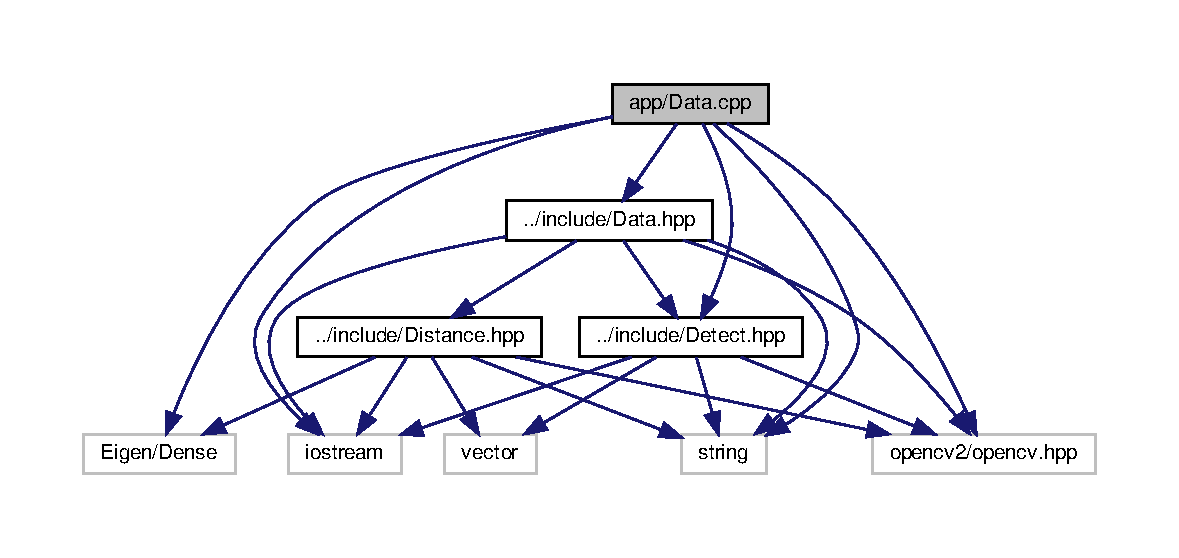
\includegraphics[width=350pt]{Data_8cpp__incl}
\end{center}
\end{figure}


\subsection{Detailed Description}
\hyperlink{classData}{Data} Class Definition. 

\begin{DoxyAuthor}{Author}
Aditya Jadhav (\href{mailto:amjadhav@umd.edu}{\tt amjadhav@umd.\+edu}) 

Abhishek Nalawade (\href{mailto:abhi1793@umd.edu}{\tt abhi1793@umd.\+edu}) 
\end{DoxyAuthor}
\begin{DoxyVersion}{Version}
0.\+1 
\end{DoxyVersion}
\begin{DoxyDate}{Date}
2021-\/10-\/15
\end{DoxyDate}
\begin{DoxyCopyright}{Copyright}
Copyright (c) 2021 
\end{DoxyCopyright}

\hypertarget{Detect_8cpp}{}\section{app/\+Detect.cpp File Reference}
\label{Detect_8cpp}\index{app/\+Detect.\+cpp@{app/\+Detect.\+cpp}}


\hyperlink{classDetect}{Detect} Class Definition.  


{\ttfamily \#include \char`\"{}../include/\+Detect.\+hpp\char`\"{}}\newline
{\ttfamily \#include $<$iostream$>$}\newline
{\ttfamily \#include $<$vector$>$}\newline
{\ttfamily \#include $<$string$>$}\newline
{\ttfamily \#include $<$opencv2/opencv.\+hpp$>$}\newline
Include dependency graph for Detect.\+cpp\+:
\nopagebreak
\begin{figure}[H]
\begin{center}
\leavevmode
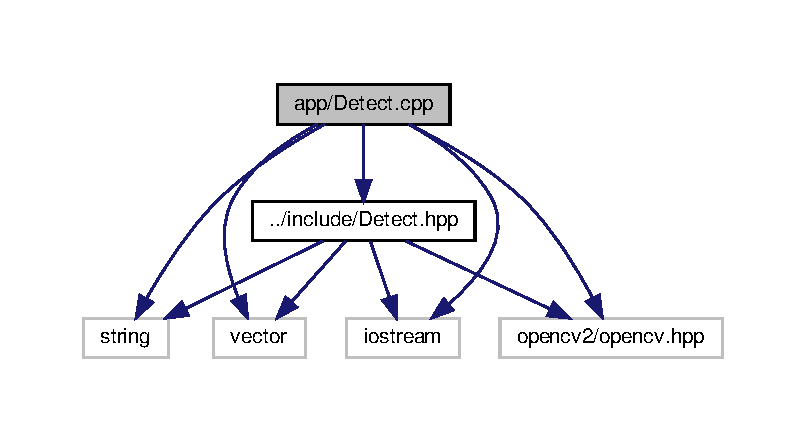
\includegraphics[width=350pt]{Detect_8cpp__incl}
\end{center}
\end{figure}


\subsection{Detailed Description}
\hyperlink{classDetect}{Detect} Class Definition. 

\begin{DoxyAuthor}{Author}
Aditya Jadhav (\href{mailto:amjadhav@umd.edu}{\tt amjadhav@umd.\+edu}) 

Abhishek Nalawade (\href{mailto:abhi1793@umd.edu}{\tt abhi1793@umd.\+edu}) 
\end{DoxyAuthor}
\begin{DoxyVersion}{Version}
0.\+1 
\end{DoxyVersion}
\begin{DoxyDate}{Date}
2021-\/10-\/17
\end{DoxyDate}
\begin{DoxyCopyright}{Copyright}
Copyright (c) 2021 
\end{DoxyCopyright}

\hypertarget{Distance_8cpp}{}\section{app/\+Distance.cpp File Reference}
\label{Distance_8cpp}\index{app/\+Distance.\+cpp@{app/\+Distance.\+cpp}}


\hyperlink{classDistance}{Distance} Class Definition.  


{\ttfamily \#include \char`\"{}../include/\+Distance.\+hpp\char`\"{}}\newline
{\ttfamily \#include $<$iostream$>$}\newline
{\ttfamily \#include $<$string$>$}\newline
{\ttfamily \#include $<$fstream$>$}\newline
{\ttfamily \#include $<$opencv2/opencv.\+hpp$>$}\newline
Include dependency graph for Distance.\+cpp\+:
\nopagebreak
\begin{figure}[H]
\begin{center}
\leavevmode
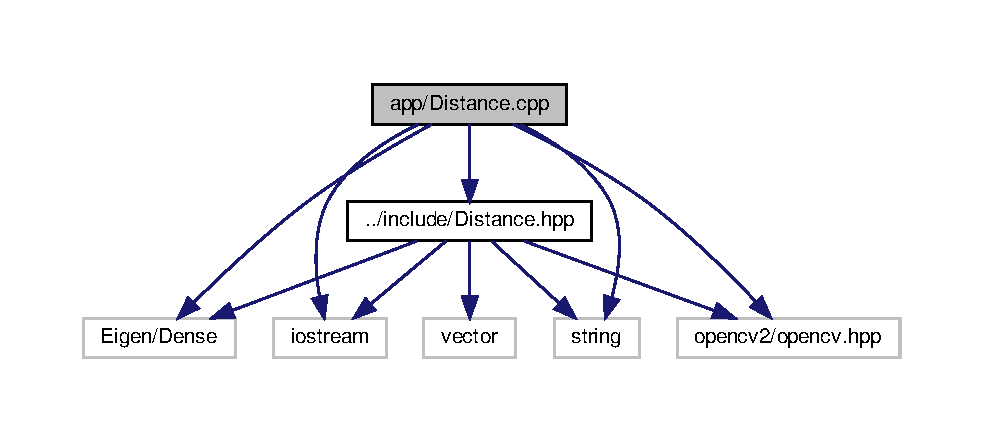
\includegraphics[width=350pt]{Distance_8cpp__incl}
\end{center}
\end{figure}


\subsection{Detailed Description}
\hyperlink{classDistance}{Distance} Class Definition. 

\begin{DoxyAuthor}{Author}
Aditya Jadhav (\href{mailto:amjadhav@umd.edu}{\tt amjadhav@umd.\+edu}) 

Abhishek Nalawade (\href{mailto:abhi1793@umd.edu}{\tt abhi1793@umd.\+edu}) 
\end{DoxyAuthor}
\begin{DoxyVersion}{Version}
0.\+1 
\end{DoxyVersion}
\begin{DoxyDate}{Date}
2021-\/10-\/17
\end{DoxyDate}
\begin{DoxyCopyright}{Copyright}
Copyright (c) 2021 
\end{DoxyCopyright}

\hypertarget{Data_8hpp}{}\section{include/\+Data.hpp File Reference}
\label{Data_8hpp}\index{include/\+Data.\+hpp@{include/\+Data.\+hpp}}


\hyperlink{classData}{Data} Class Declaration.  


{\ttfamily \#include $<$string$>$}\newline
{\ttfamily \#include $<$iostream$>$}\newline
{\ttfamily \#include \char`\"{}../include/\+Distance.\+hpp\char`\"{}}\newline
{\ttfamily \#include \char`\"{}../include/\+Detect.\+hpp\char`\"{}}\newline
{\ttfamily \#include $<$opencv2/opencv.\+hpp$>$}\newline
Include dependency graph for Data.\+hpp\+:
\nopagebreak
\begin{figure}[H]
\begin{center}
\leavevmode
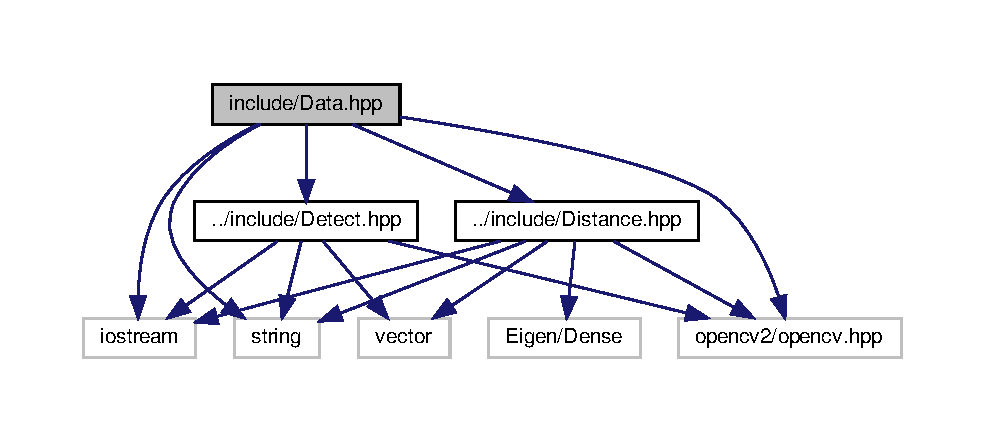
\includegraphics[width=350pt]{Data_8hpp__incl}
\end{center}
\end{figure}
This graph shows which files directly or indirectly include this file\+:
\nopagebreak
\begin{figure}[H]
\begin{center}
\leavevmode
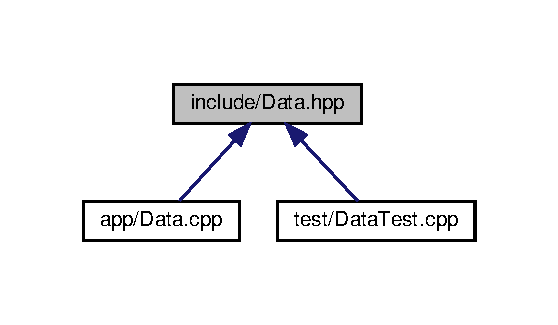
\includegraphics[width=268pt]{Data_8hpp__dep__incl}
\end{center}
\end{figure}
\subsection*{Classes}
\begin{DoxyCompactItemize}
\item 
class \hyperlink{classData}{Data}
\begin{DoxyCompactList}\small\item\em \hyperlink{classData}{Data} class includes methods to get the input data and a method to put bounging boxes around the detected humans. \end{DoxyCompactList}\end{DoxyCompactItemize}


\subsection{Detailed Description}
\hyperlink{classData}{Data} Class Declaration. 

\begin{DoxyAuthor}{Author}
Aditya Jadhav (\href{mailto:amjadhav@umd.edu}{\tt amjadhav@umd.\+edu}) 

Abhishek Nalawade (\href{mailto:abhi1793@umd.edu}{\tt abhi1793@umd.\+edu}) 
\end{DoxyAuthor}
\begin{DoxyVersion}{Version}
0.\+1 
\end{DoxyVersion}
\begin{DoxyDate}{Date}
2021-\/10-\/15
\end{DoxyDate}
\begin{DoxyCopyright}{Copyright}
Copyright (c) 2021 
\end{DoxyCopyright}

\hypertarget{Detect_8hpp}{}\section{include/\+Detect.hpp File Reference}
\label{Detect_8hpp}\index{include/\+Detect.\+hpp@{include/\+Detect.\+hpp}}


\hyperlink{classDetect}{Detect} Class Declaration.  


{\ttfamily \#include $<$string$>$}\newline
{\ttfamily \#include $<$vector$>$}\newline
{\ttfamily \#include $<$iostream$>$}\newline
{\ttfamily \#include $<$opencv2/opencv.\+hpp$>$}\newline
Include dependency graph for Detect.\+hpp\+:
\nopagebreak
\begin{figure}[H]
\begin{center}
\leavevmode
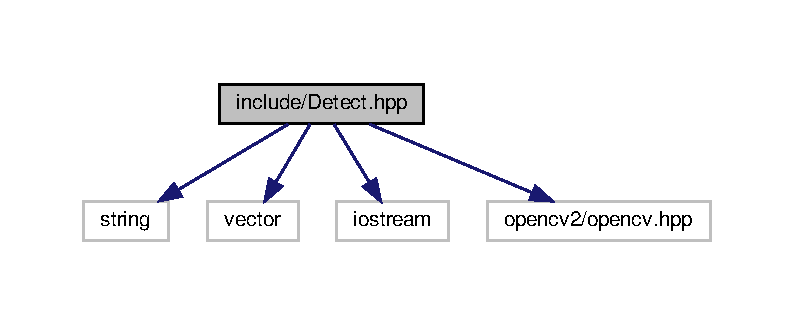
\includegraphics[width=350pt]{Detect_8hpp__incl}
\end{center}
\end{figure}
This graph shows which files directly or indirectly include this file\+:
\nopagebreak
\begin{figure}[H]
\begin{center}
\leavevmode
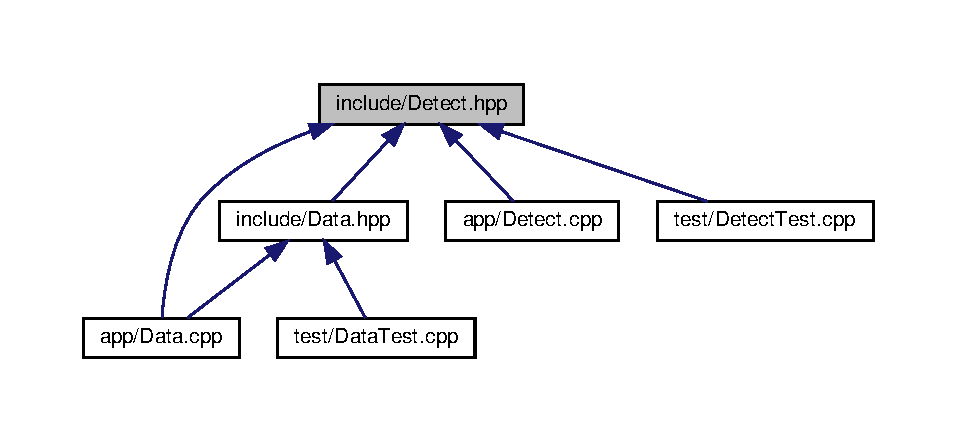
\includegraphics[width=350pt]{Detect_8hpp__dep__incl}
\end{center}
\end{figure}
\subsection*{Classes}
\begin{DoxyCompactItemize}
\item 
class \hyperlink{classDetect}{Detect}
\begin{DoxyCompactList}\small\item\em \hyperlink{classDetect}{Detect} class uses a pre-\/trained S\+VM model from open\+CV to detect humans in the input frames and return bounding box co-\/ordinates. \end{DoxyCompactList}\end{DoxyCompactItemize}


\subsection{Detailed Description}
\hyperlink{classDetect}{Detect} Class Declaration. 

\begin{DoxyAuthor}{Author}
Aditya Jadhav (\href{mailto:amjadhav@umd.edu}{\tt amjadhav@umd.\+edu}) 

Abhishek Nalawade (\href{mailto:abhi1793@umd.edu}{\tt abhi1793@umd.\+edu}) 
\end{DoxyAuthor}
\begin{DoxyVersion}{Version}
0.\+1 
\end{DoxyVersion}
\begin{DoxyDate}{Date}
2021-\/10-\/17
\end{DoxyDate}
\begin{DoxyCopyright}{Copyright}
Copyright (c) 2021 
\end{DoxyCopyright}

\hypertarget{Distance_8hpp}{}\section{include/\+Distance.hpp File Reference}
\label{Distance_8hpp}\index{include/\+Distance.\+hpp@{include/\+Distance.\+hpp}}


\hyperlink{classDistance}{Distance} Class Declaration.  


{\ttfamily \#include $<$Eigen/\+Dense$>$}\newline
{\ttfamily \#include $<$string$>$}\newline
{\ttfamily \#include $<$vector$>$}\newline
{\ttfamily \#include $<$iostream$>$}\newline
{\ttfamily \#include $<$opencv2/opencv.\+hpp$>$}\newline
Include dependency graph for Distance.\+hpp\+:
\nopagebreak
\begin{figure}[H]
\begin{center}
\leavevmode
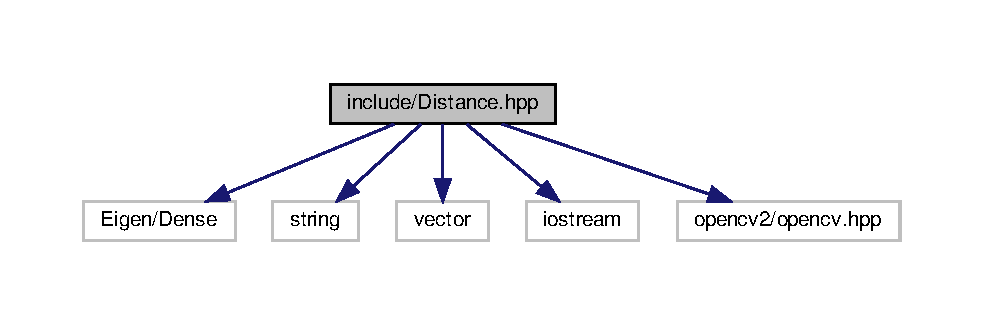
\includegraphics[width=350pt]{Distance_8hpp__incl}
\end{center}
\end{figure}
This graph shows which files directly or indirectly include this file\+:
\nopagebreak
\begin{figure}[H]
\begin{center}
\leavevmode
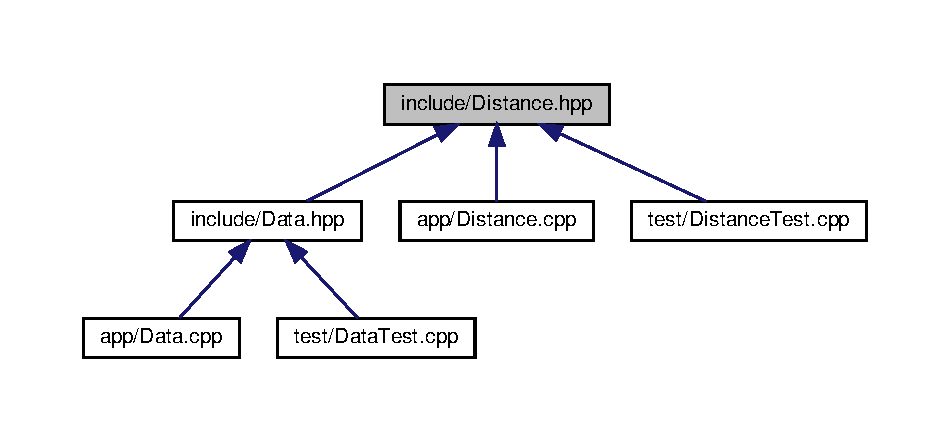
\includegraphics[width=350pt]{Distance_8hpp__dep__incl}
\end{center}
\end{figure}
\subsection*{Classes}
\begin{DoxyCompactItemize}
\item 
class \hyperlink{classDistance}{Distance}
\begin{DoxyCompactList}\small\item\em \hyperlink{classDistance}{Distance} class to provide the pixel to SI units conversion as well as the Transformation between Camera frame and Robot frame. \end{DoxyCompactList}\end{DoxyCompactItemize}


\subsection{Detailed Description}
\hyperlink{classDistance}{Distance} Class Declaration. 

\begin{DoxyAuthor}{Author}
Aditya Jadhav (\href{mailto:amjadhav@umd.edu}{\tt amjadhav@umd.\+edu}) 

Abhishek Nalawade (\href{mailto:abhi1793@umd.edu}{\tt abhi1793@umd.\+edu}) 
\end{DoxyAuthor}
\begin{DoxyVersion}{Version}
0.\+1 
\end{DoxyVersion}
\begin{DoxyDate}{Date}
2021-\/10-\/17
\end{DoxyDate}
\begin{DoxyCopyright}{Copyright}
Copyright (c) 2021 
\end{DoxyCopyright}

\hypertarget{DataTest_8cpp}{}\section{test/\+Data\+Test.cpp File Reference}
\label{DataTest_8cpp}\index{test/\+Data\+Test.\+cpp@{test/\+Data\+Test.\+cpp}}


\hyperlink{classData}{Data} Class Tests.  


{\ttfamily \#include $<$gtest/gtest.\+h$>$}\newline
{\ttfamily \#include $<$string$>$}\newline
{\ttfamily \#include \char`\"{}../include/\+Data.\+hpp\char`\"{}}\newline
{\ttfamily \#include $<$opencv2/opencv.\+hpp$>$}\newline
Include dependency graph for Data\+Test.\+cpp\+:
\nopagebreak
\begin{figure}[H]
\begin{center}
\leavevmode
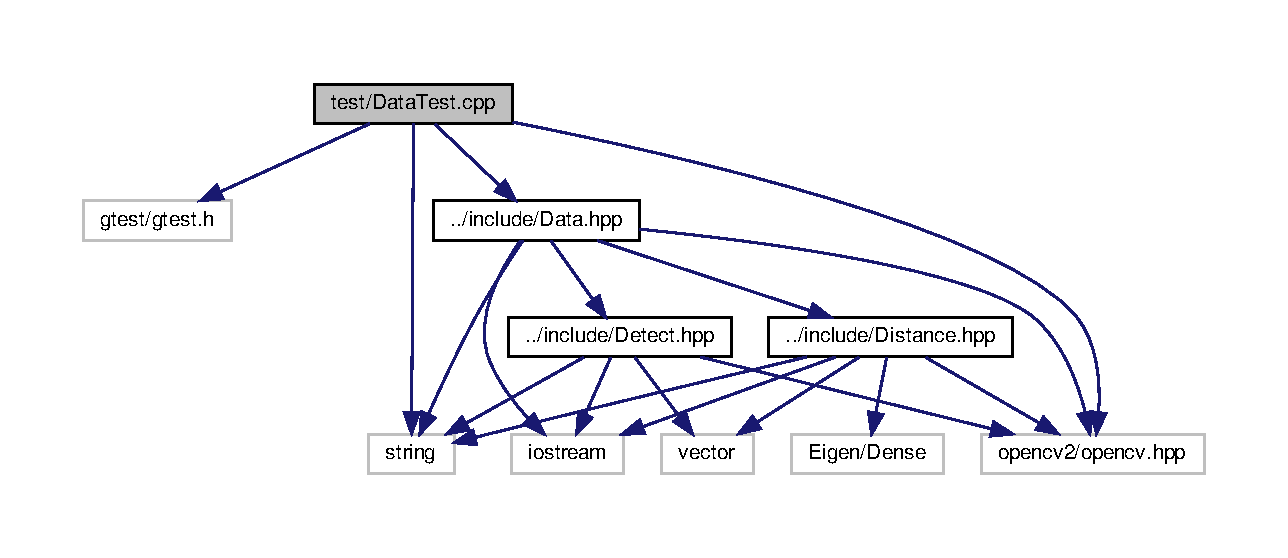
\includegraphics[width=350pt]{DataTest_8cpp__incl}
\end{center}
\end{figure}
\subsection*{Functions}
\begin{DoxyCompactItemize}
\item 
\mbox{\Hypertarget{DataTest_8cpp_a59d7b4be5232026254467d515ca7a1f0}\label{DataTest_8cpp_a59d7b4be5232026254467d515ca7a1f0}} 
\hyperlink{DataTest_8cpp_a59d7b4be5232026254467d515ca7a1f0}{T\+E\+ST} (Camera, Data\+\_\+\+Input\+\_\+\+Method\+\_\+camera\+\_\+works)
\begin{DoxyCompactList}\small\item\em Test to validate if the camera cannot be opened. \end{DoxyCompactList}\item 
\mbox{\Hypertarget{DataTest_8cpp_a0b9f2c4532178433770ef45d47ad7b37}\label{DataTest_8cpp_a0b9f2c4532178433770ef45d47ad7b37}} 
\hyperlink{DataTest_8cpp_a0b9f2c4532178433770ef45d47ad7b37}{T\+E\+ST} (Video, Data\+\_\+\+Input\+\_\+as\+\_\+\+File\+\_\+does\+\_\+not\+\_\+exist)
\begin{DoxyCompactList}\small\item\em Test to verify the video file does not exist and no frame is read. \end{DoxyCompactList}\item 
\mbox{\Hypertarget{DataTest_8cpp_a1e2a145893ac4ad978fcb0d84fd1e2ac}\label{DataTest_8cpp_a1e2a145893ac4ad978fcb0d84fd1e2ac}} 
\hyperlink{DataTest_8cpp_a1e2a145893ac4ad978fcb0d84fd1e2ac}{T\+E\+ST} (Processing, Processed\+\_\+\+Image\+\_\+\+Rows)
\begin{DoxyCompactList}\small\item\em Test to verify the number of rows after preprocessing. \end{DoxyCompactList}\end{DoxyCompactItemize}


\subsection{Detailed Description}
\hyperlink{classData}{Data} Class Tests. 

\begin{DoxyAuthor}{Author}
Aditya Jadhav (\href{mailto:amjadhav@umd.edu}{\tt amjadhav@umd.\+edu}) 

Abhishek Nalawade (\href{mailto:abhi1793@umd.edu}{\tt abhi1793@umd.\+edu}) 
\end{DoxyAuthor}
\begin{DoxyVersion}{Version}
0.\+1 
\end{DoxyVersion}
\begin{DoxyDate}{Date}
2021-\/10-\/17
\end{DoxyDate}
\begin{DoxyCopyright}{Copyright}
Copyright (c) 2021 
\end{DoxyCopyright}

\hypertarget{DetectTest_8cpp}{}\section{test/\+Detect\+Test.cpp File Reference}
\label{DetectTest_8cpp}\index{test/\+Detect\+Test.\+cpp@{test/\+Detect\+Test.\+cpp}}


\hyperlink{classDetect}{Detect} Class Tests.  


{\ttfamily \#include $<$gtest/gtest.\+h$>$}\newline
{\ttfamily \#include \char`\"{}../include/\+Detect.\+hpp\char`\"{}}\newline
{\ttfamily \#include $<$opencv2/opencv.\+hpp$>$}\newline
Include dependency graph for Detect\+Test.\+cpp\+:
\nopagebreak
\begin{figure}[H]
\begin{center}
\leavevmode
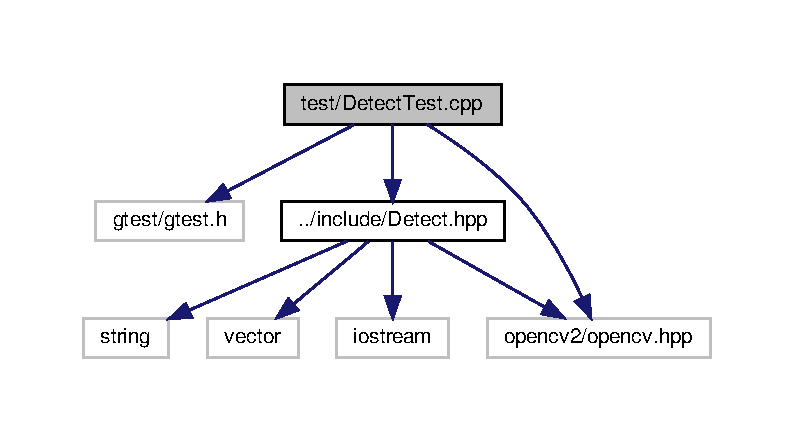
\includegraphics[width=350pt]{DetectTest_8cpp__incl}
\end{center}
\end{figure}
\subsection*{Functions}
\begin{DoxyCompactItemize}
\item 
\mbox{\Hypertarget{DetectTest_8cpp_a6164d059692bf99e55eb9dfaed457406}\label{DetectTest_8cpp_a6164d059692bf99e55eb9dfaed457406}} 
\hyperlink{DetectTest_8cpp_a6164d059692bf99e55eb9dfaed457406}{T\+E\+ST} (Detect\+\_\+test, checking\+\_\+detected\+\_\+human)
\begin{DoxyCompactList}\small\item\em Test to verify the size of the bounding box. \end{DoxyCompactList}\item 
\mbox{\Hypertarget{DetectTest_8cpp_ad0f598c7686aa81f55ea48f93ded50cd}\label{DetectTest_8cpp_ad0f598c7686aa81f55ea48f93ded50cd}} 
\hyperlink{DetectTest_8cpp_ad0f598c7686aa81f55ea48f93ded50cd}{T\+E\+ST} (Bounding\+\_\+box\+\_\+test, checking\+\_\+height)
\begin{DoxyCompactList}\small\item\em Construct a new T\+E\+ST object. \end{DoxyCompactList}\end{DoxyCompactItemize}


\subsection{Detailed Description}
\hyperlink{classDetect}{Detect} Class Tests. 

\begin{DoxyAuthor}{Author}
Aditya Jadhav (\href{mailto:amjadhav@umd.edu}{\tt amjadhav@umd.\+edu}) 

Abhishek Nalawade (\href{mailto:abhi1793@umd.edu}{\tt abhi1793@umd.\+edu}) 
\end{DoxyAuthor}
\begin{DoxyVersion}{Version}
0.\+1 
\end{DoxyVersion}
\begin{DoxyDate}{Date}
2021-\/10-\/17
\end{DoxyDate}
\begin{DoxyCopyright}{Copyright}
Copyright (c) 2021 
\end{DoxyCopyright}

\hypertarget{DistanceTest_8cpp}{}\section{test/\+Distance\+Test.cpp File Reference}
\label{DistanceTest_8cpp}\index{test/\+Distance\+Test.\+cpp@{test/\+Distance\+Test.\+cpp}}


\hyperlink{classDistance}{Distance} Class Tests.  


{\ttfamily \#include $<$gtest/gtest.\+h$>$}\newline
{\ttfamily \#include \char`\"{}../include/\+Distance.\+hpp\char`\"{}}\newline
{\ttfamily \#include $<$opencv2/opencv.\+hpp$>$}\newline
Include dependency graph for Distance\+Test.\+cpp\+:
\nopagebreak
\begin{figure}[H]
\begin{center}
\leavevmode
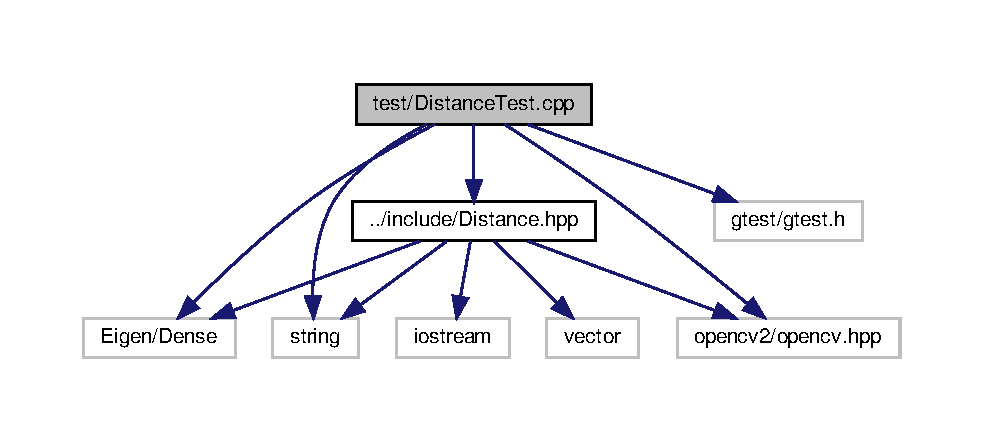
\includegraphics[width=350pt]{DistanceTest_8cpp__incl}
\end{center}
\end{figure}
\subsection*{Functions}
\begin{DoxyCompactItemize}
\item 
\mbox{\Hypertarget{DistanceTest_8cpp_ad7d81996cf31d4380cdbdd66d5e5275a}\label{DistanceTest_8cpp_ad7d81996cf31d4380cdbdd66d5e5275a}} 
\hyperlink{DistanceTest_8cpp_ad7d81996cf31d4380cdbdd66d5e5275a}{T\+E\+ST} (S\+I\+Distance, Tranform\+\_\+check)
\begin{DoxyCompactList}\small\item\em Test to verify if the correct tranformation is applied. \end{DoxyCompactList}\end{DoxyCompactItemize}


\subsection{Detailed Description}
\hyperlink{classDistance}{Distance} Class Tests. 

\begin{DoxyAuthor}{Author}
Aditya Jadhav (\href{mailto:amjadhav@umd.edu}{\tt amjadhav@umd.\+edu}) 

Abhishek Nalawade (\href{mailto:abhi1793@umd.edu}{\tt abhi1793@umd.\+edu}) 
\end{DoxyAuthor}
\begin{DoxyVersion}{Version}
0.\+1 
\end{DoxyVersion}
\begin{DoxyDate}{Date}
2021-\/10-\/17
\end{DoxyDate}
\begin{DoxyCopyright}{Copyright}
Copyright (c) 2021 
\end{DoxyCopyright}

%--- End generated contents ---

% Index
\backmatter
\newpage
\phantomsection
\clearemptydoublepage
\addcontentsline{toc}{chapter}{Index}
\printindex

\end{document}
